% Fig. 6 — Ablation bar chart (ILLUSTRATIVE placeholder data)
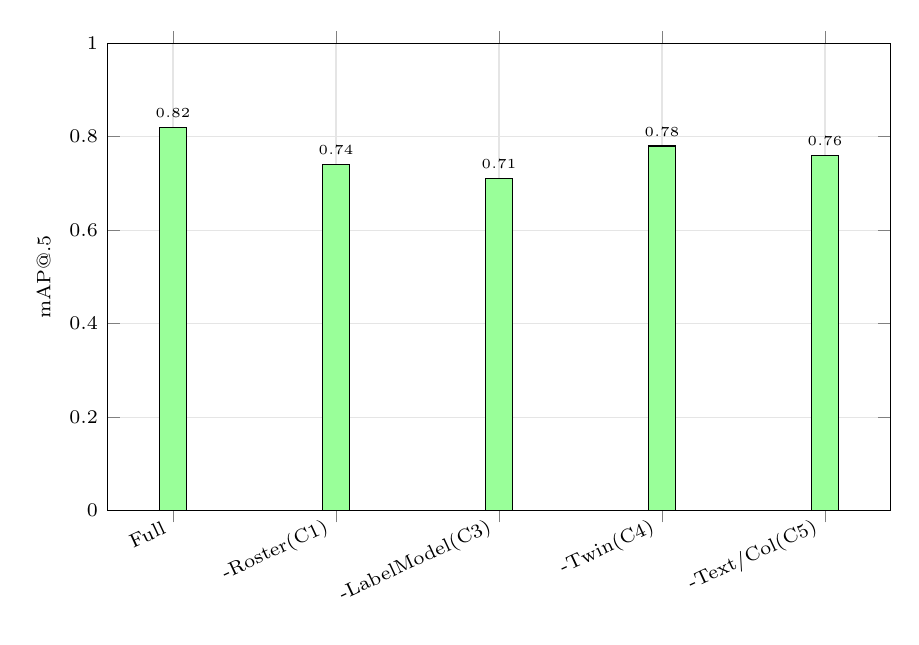
\begin{tikzpicture}
\begin{axis}[
  width=0.95\columnwidth, height=0.62\columnwidth,
  ybar, bar width=10pt,
  ymin=0, ymax=1, ylabel={mAP@.5},
  symbolic x coords={Full,-Roster(C1),-LabelModel(C3),-Twin(C4),-Text/Col(C5)},
  xtick=data, x tick label style={rotate=25, anchor=east, font=\scriptsize},
  tick label style={font=\scriptsize}, label style={font=\scriptsize},
  nodes near coords, nodes near coords style={font=\tiny},
  grid=both, grid style={gray!20},
]
% PLACEHOLDER deltas -- replace with measured values
\addplot[fill=green!40] coordinates
  {(Full,0.82) (-Roster(C1),0.74) (-LabelModel(C3),0.71)
   (-Twin(C4),0.78) (-Text/Col(C5),0.76)};
\end{axis}
\end{tikzpicture}
